\subsection{Algorithm Implementation in the Safety Annex}
\label{sec:impl}
%%%%%%%%%%%%%%%%%%%%%%%%%%%%%%%%%%%%%%%%%%%%%%%%%
%%%%%%%%%%%%%%%%%%%%            ALGORITHM DETAILS
%In the formalism section, we viewed the problem from the perspective of an arbitary guarantee in the model that can potentially be violated. This resulted in explicit faults at the leaf level and violated guarantees (``nondeterministic faults") at the middle/top layers. Each MCS generated at each level gives insight into the system at that level. In this section, we describe the implementation of compositional generation of minimal cut sets. %Minimal cut sets traditionally contain explicitly defined faults as elements; to this end, we implemented a compositional mapping from explicit faults to the guarantees they violate. The end result are the minimal cut sets that contribute to a violation of the top level safety property. 
In the formalism, any guarantee in the model had an associated fault activation literal and could be unconstrained. In the implementation, we rely on the fault model created in the safety annex to dictate which guarantees can be violated and how they may fail. Each explicit fault defined in the safety annex is added to the Lustre program as are assocated fault activation literals~\cite{Stewart17:IMBSA,stewart2020safety}. This corresponds to the $f_i$ and $\mathit{af}_i$ described in Section~\ref{sec:formalization}. 

\begin{figure}[h!]
	%\vspace{-2em}
	\begin{center}
		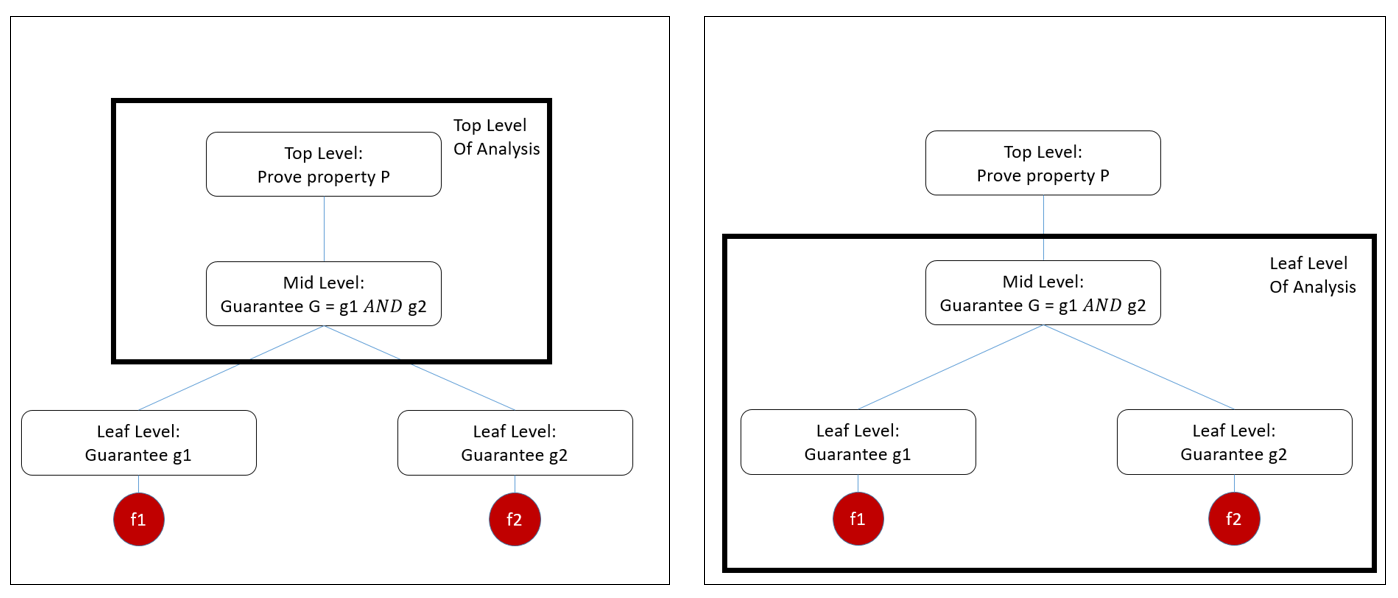
\includegraphics[width=0.7\textwidth]{images/twoLevels.PNG}
	\end{center}
	\vspace{-2em}
	\caption{Illustration of Two Layers of Analysis}
	\label{fig:layers}
\end{figure}

The \aivcalg algorithm requires  specific equations in the Lustre model to be flagged for consideration in the analysis; these we call \emph{IVC algorithm elements}. All equations in the model can be used as IVC algorithm elements or one can specify directly the equations to consider. In this implementation, the IVC algorithm elements are added differently depending on the layer. In the leaf architectural level, fault activation literals are added to the IVC algorithm elements and are constrained to {\em false}. In middle or top layers, supporting guarantees are added. This is shown in Figure~\ref{fig:layers}. 

The figure shows an arbitrary architecture with two analysis layers: top and leaf. The top layer analysis adds $G$ as IVC algorithm element; the leaf layer analysis adds $f_1$ and $f_2$. 

A requirement of the hitting set algorithm is that to find all MCSs, all MUSs must be known. Ghassabani et al.~\cite{Ghassabani2017EfficientGO} showed that finding all MIVCs is as hard as model checking. It is a requirement of this analysis that all MIVCs are found. Once the MIVC analysis is complete for a property at a given layer, a hitting set algorithm is used to generate the related MCSs~\cite{gainer2017minimal}. Depending on the layer of analysis, the MCSs contain either guarantees (mid layer) or fault activation literals (leaf layer).

%For a safety property $P$, the set of all MCSs are understood as $\lor^{n}_{i=1} MCS_i(P)$; intuitively, this means if all constraints found in any single MCS are removed from the constraint system, $\neg P$ is satisfied. For each element $gf_j \in MCS_i$, this is understood as $\land^{m}_{i=1} gf_i$ and speaks to the minimality of the correction set. Thus the MCSs form a disjunctive normal formula over the safety property at that layer. As the proof proceeds down the hierarchy, each of the subcomponent guarantees become a property to be proven and thus MIVCs/MCSs are generated. The composition of the MCSs consists of replacing a contract in a higher layer MCS with the disjunctive normal formula of its own MCSs. After all replacements have been made, the system property formula is converted back into disjunctive normal form. 

\begin{algorithm}[h]
\SetKwFunction{Resolve}{resolve}
 \SetKwProg{Fn}{Function}{:}{}

	$R \gets \mathit{\amcs(P)} = \lor_{i=1}^n \mathit{MCS}_i$\\
	where $\mathit{MCS}_i = \land_{j=1}^m \mathit{gf_j}$\\
	\Fn{\Resolve{$R$}}{
		
		\For{$\forall$ OR-node in $R$}{
			\For{$\forall \mathit{gf_j}$ in OR-node}{
				\eIf{ $\exists MCS(gf_j)$ }{
				$R \gets$ replace $gf_j$ in $R$ with $\mathit{\amcs(gf_j)}$\;
				\Resolve($\mathit{\amcs(gf_j)}$)\;
			}{
				$R \gets $ replace $\mathit{gf_j}$ in $R$ with $\mathit{af_j}$\;	
			} 
			}
		}
		convert $R$ to DNF 
	}
	\caption{Compose Results}
	\label{alg:compose}
\end{algorithm}

The composition of these results is performed top down and shown in Algorithm~\ref{alg:compose}. For each guarantee found in an MCS, a replacement is made with the guarantee's own MCSs. This is done recursively until all replacements have been made (line 7, 8 of Algorithm~\ref{alg:compose}). If on the other hand there are no MCSs for a given guarantee, that guarantee is replaced by its associated fault activation literal (line 10). At the leaf level of analysis, no guarantees have associated MCSs (there are no children properties) and thus reaches the end of recursion. At that time, the formula is converted back into disjunctive normal form of fault activation literals to finish the translation into the traditional fault tree (line 11). 

Algorithm~\ref{alg:compose} provides the outline for the general case of composing fault forests: for each each property in a layer of analysis, the algorithm is called. Each property may have a corresponding fault tree. The collection of fault trees associated with each property make the forest. In the next subsection, we describe how this general algorithm is adjusted.

The number of replacements $r$ that are made for a single property $P$ are constrained by the number of minimal cut sets there are for each of the $\alpha$ contracts within the initial MCS. We call the set of all minimal cut sets for a contract $g$: $\mathit{Cut(g)}$. The following formula defines an upper bound on the number of replacements. 

\begin{lemma}
The number of replacements $r$ is bounded by the following formula:
\begin{gather}
\label{eq:bound}
  r \leq {\displaystyle \sum_{i=1}^{\alpha} }({\displaystyle \prod_{j=1}^{i} |\mathit{Cut(g_j)}|})  
\end{gather}
\begin{proof}
Assume there exists a $g_i \in \mathit{MCS(P)}$. The number of replacements made for $g_i$ is at most $|\mathit{Cut(g_i)}|$. Iteratively perform this replacement for all $\alpha$ contracts in $\mathit{MCS(P)}$. In the worst case, $N = |\mathit{Cut(g_1)}| \times |\mathit{Cut(g_2)}| \times \cdots \times |\mathit{Cut(g_\alpha)}|$ replacements are made per $n$ layers of analysis.
\label{lemma:bound}
\end{proof}
\end{lemma}





\begin{theorem}
Algorithm~\ref{alg:compose} terminates
\begin{proof}
No infinite sets are generated by the \aivcalg or minimal hitting set algorithms~\cite{Ghassabani2017EfficientGO,murakami2013efficient}; therefore, every MCS produced is finite. Then by Lemma~\ref{lemma:bound}, the recursion is bounded by $N$ per layer of analysis.
\end{proof}
\end{theorem}

Given that the growth of the DNF formula can grow quite quickly in the worst case, we implemented strategies to prune the size of the intermediate fault trees. 


\subsection{Pruning to Address Scalability}
The safety annex provides the capability to specify a type of verification in what is called a \textit{fault hypothesis statement}. These come in two forms: maximum number of faults or probabilistic analysis. Algorithm~\ref{alg:compose} is the general approach, but the implementation changes slightly depending on which form of analysis is being performed. This pruning improves performance and diminishes the problem of combinatorial explosion in the size of minimal cut sets for larger models. 

\textbf{Guarantees with no associated faults} If a guarantee is found in a minimal correction set and no fault has been defined in the model that can violate it, this minimal correction set (and hence the entire subtree) is pruned.

\textbf{Max $n$ faults analysis} The max $n$ fault hypothesis in the safety annex restricts the number of faults that can be independently active simultaneously. This statement restricts the cardinality of minimal cut sets generated to $n$. If the number of elements in an MCS exceeds the threshold of the hypothesis statement, that MCS is eliminated from consideration and its subtree is pruned.


\textbf{Probabilistic analysis pruning} A probabilistic hypothesis statement restricts the cut sets by use of a probabilistic threshold. Assuming independence between faults, any cut sets with combined probability higher than the given probabilistic threshold are removed from consideration. The allowable combinations of faults are calculated before Algorithm~\ref{alg:compose} begins; this allows for dynamic pruning of minimal correction sets. If the fault activation literals within an MCS are not a subset of any allowable combination, that MCS is pruned from the formula. 

To access the algorithm implementation or example models, see the repository~\cite{SAGithub}. 








\begin{comment}

\setcounter{AlgoLine}{0}
\Fn{\FindMIVCs{}}{
	\While{$\mathit{Unexplored} \neq \emptyset$}{
		%$U_{max} \gets$ a maximal $U_{max} \in \mathit{Unexplored}$\;
		$U_{\mathit{max}} \gets $ a maximal set $\in \mathit{Unexplored}$\;
        \eIf{$\Solve(I,U_{\mathit{max}},P)$}{
			$U_{\mathit{IVC}} \gets \approx((I,U_{\mathit{max}}), P)$\;
			$\Shrink(U_{\mathit{IVC}})$\;
		}{
			$\mathit{Unexplored} \gets \mathit{Unexplored} \setminus \mathit{Sub}(U_{\mathit{max}})$\;			
		}
		\While{$\mathit{shrinkingQueue}$ is not empty}{
			$\mathit{U} \gets \Dequeue(\mathit{shrinkingQueue})$\;
			$\Shrink(\mathit{U})$\;
		}
	}
}


The transformation of MIVCs to MinCutSets can only be performed if \emph{all} MIVCs have been generated. It is a requirement of the minimal hitting set algorithm that all MUSs are used to find the MCSs~\cite{liffiton2016fast,gainer2017minimal,murakami2013efficient}. Thus, once all MIVCs have been found and the minimal hitting set algorithm has completed, the MinCutSet generation can begin. 

The MinCutSet generation algorithm begins with a list of MCSs specific to a property. These MCSs may contain a mixture of fault activation literals constrained to \textit{false} and subcomponent contracts constrained to \textit{true}. We remove all constraints from each MCS and call the resulting sets $I$, for \textit{Intermediate} set.  For each of those contracts in $I$, we check to see if we have previously obtained a MinCutSet for that contract. If so, replacement is performed. If not, we recursively call this algorithm to obtain the list of all MinCutSets associated with this subcomponent contract. At a certain point, there will be no more contracts in the set $I$ in which case we have a minimal cut set for the current property. The reason is because at the lowest levels of the system, the only model elements used in the constraint system analyzed by the \aivcalg algorithm are faults. Thus when the contracts at the lowest level are the safety properties for the \aivcalg algorithm, the MUSs contain only faults (likewise the MCSs). When this cut set is obtained for the lowest level properties, it is stored in a lookup table keyed by the given property. Algorithm~\ref{alg:generation_alg} describes this process.


\begin{algorithm}[h]
\SetKwFunction{FMain}{replace}
 \SetKwProg{Fn}{Function}{:}{}

	\Fn{\FMain{$P$}}{
		$List(I)$:= $List(MCS)$ for $P$ with all constraints removed \;
		\For{all $I \in List(I)$}{
			\eIf{there exists contracts $g \in I$}{
				\For{all constrained contracts $g \in I$}{
					\eIf{there exists $MinCutSets$ for $g$ in lookup table}{
						\For{all $minCut(g)$}{
							$I_{repl} = I$ \;
							$I_{repl} :=$ replace $g$ with $minCut(g)$ \;
							add $I_{repl}$ to $List(I)$ \;
						} %end for all cut sets of g
					}{
						replace($g$) \;
					} % end else if no cut sets in lookup table
				} % end for all constrained contracts in I
			}{
				add $I$ as $minCut(g)$ for $P$ \;
			} %end else if there exists contracts in I
		}%end for all I in list(I)
	}
%	\caption{Minimal Cut Set Generation Algorithm}
	\caption{MinCutSets Generation Algorithm}
	\label{alg:generation_alg}
\end{algorithm}

The number of replacements $R$ that are made in this algorithm are constrained by the number of minimal cut sets there are for all $\alpha$ contracts within the initial MCS. 

We call the set of all minimal cut sets for a contract $g$: $Cut(g)$. The following formula defines an upper bound on the number of replacements. The validity of this statement follows directly from the general multiplicative combinatorial principle. The number of replacements $R$ is bounded by the following formula:
\begin{equation}
\label{eq:bound}
  R \leq {\displaystyle \sum_{i=1}^{\alpha} }({\displaystyle \prod_{j=1}^{i} |Cut(g_j)|})  
\end{equation}


It is also important to note that the cardinality of $List(I)$ is bounded, i.e. the algorithm terminates. Every new $I$ that is generated through some replacement of a contract with its minimal cut set is added to $List(I)$ in order to continue the replacement process for all contracts in $I$. Adding to this set requires proof regarding termination.
\begin{theorem}
Algorithm~\ref{alg:generation_alg} terminates
\begin{proof}
No infinite sets are generated by the \aivcalg or minimal hitting set algorithms~\cite{Ghassabani2017EfficientGO,murakami2013efficient}; therefore, every MCS produced is finite. Thus, every $MinCutSet$ of every contract $g$ is finite. Furthermore, a bound exists on the number of additional intermediate sets $I$ that are added to $List(I)$: \\
$|List(I)| \leq R$ (Equation~\ref{eq:bound}).
\end{proof}
\end{theorem}

The reason for this upper bound is that for a contract $g_1$ in MCS, we make $|Cut(g_1)|$ replacements and add the resulting lists to $List(I)$. Then we move to the next contract $g_2$ in $I$. We must additionally make $|Cut(g_1)| \times |Cut(g_2)|$ replacements and add all of these resulting lists to $List(I)$, and so on throughout all contracts. Through the use of basic combinatorial principles, we end with the above formula for the upper bound on the number of additional intermediate sets.


\subsubsection{Pruning to Address Scalability}
The MinCutSets are filtered during this process based on a fault hypothesis given before analysis begins. The Safety Annex provides the capability to specify a type of verification in what is called a \textit{fault hypothesis statement}. These come in two forms: maximum number of faults or probabilistic analysis. Algorithm~\ref{alg:generation_alg} is the general approach, but the implementation changes slightly depending on which form of analysis is being performed. This pruning improves performance and diminishes the problem of combinatorial explosions in the size of minimal cut sets for larger models. \\

\textbf{Max $N$ Analysis Pruning} This statement restricts the number of faults that can be independently active simultaneously and verification is run with this restriction present. For example, if a max 2 fault hypothesis is specified, two or fewer faults may be active at once. In terms of minimal cut sets, this statement restricts the cardinality of minimal cut sets generated.

If the number of faults in an intermediate set $I$ exceeds the threshold $N$, any further replacement of remaining contracts in that intermediate set can never decrease the total number of faults in $I$; therefore, this intermediate set is eliminated from consideration.\\

\textbf{Probabilistic Analysis Pruning} The second type of hypothesis statement restricts the cut sets by use of a probabilistic threshold. Any cut sets with combined probability higher than the given probabilistic threshold are removed from consideration. The allowable combinations of faults are calculated before the transformation algorithm begins; this allows for a pruning of intermediate sets during the transformation. If the faults within an intermediate set are not a subset of any allowable combination, that intermediate set is pruned from consideration and no further replacements are made. 

\end{comment}


